\subsection{Stäbe}
Zunächst wurde die Durchbiegung von vier verschiedenen Stäben gegen das angehängte Gewicht aufgetragen.
Bei den Stäben handelte es sich um einen Runden Stahlstab, einen Runden Aluminiumstab, einen Runden Messingstab und um einen Rechteckigen Messingstab.
Der Rechteckige Messingstab besitzt zwei unterschiedlich lange Kantenlängen. Dieser Messingstab wurde jeweils einmal so eingespannt, sodass jeweils eine der beiden Kanten nach oben zeigt.
Diese Durchbiegung in Abhängigkeit vom Gewicht ist in den Abbildungen \ref{fig:durchbiegungalu} bis \ref{fig:durchbiegungStahl} zu sehen. 
Mithilfe von den aus den Abbildungen entnommenen Steigungen wurde nach Gleichung \ref{eq:Elast} mithilfe von den Gleichungen \ref{eq:TrägKreis} und \ref{eq:TrägRecht} das Elastizitätsmodul $E$ berechnet.
Somit ergab sich unter einsetzen der in Tabelle \ref{tab:Ela} zu sehenden Werte, die ebenfalls in der Tabelle zu sehenden Werte, für das Elastizitätsmodul. 
Vergleicht man diese Werte für das Elastizitätsmodul mit Literaturwerten\footnote{Entnommen aus "Physik: für Wissenschaftler und Ingenieure" von Paul A. Tpler und Gene Mosca in der 7. Ausgabe von 2014.} Tabelle \ref{tab:ElaLit}

\begin{table}[h]
	\caption{Elastizitätsmodul E berechnet nach \ref{eq:Elast} mit allen dazu nötigen Werten}
	\begin{tabular}{|c|c|c|c|c|c|c|}
		\hline
		& a $\left[ \frac{m}{g} \right]$& b[m]& c[m] & d[m] & L[m] & E $\left[\frac{N}{m^2}  \right]$ \\
		\hline
		Aluminium Rund & 0,305 & & & 0,00297 & 0,298 & 74921967405\\
		\hline
		Messing Hochkant & 0,041 & 0,0020 & 0,0050 && 0,287 & 94293095026\\
		\hline
		Messing Quer & 0,264 & 0,0050 & 0,0020 && 0,287 & 93133852625\\
		\hline
		Messing Rund & 0,202 &&& 0,00296 & 0,295 & 111186381240\\
		\hline
		Stahl Rund & 0,114 &&& 0,00297 & 0,290 & 181538008224\\
		\hline
	\end{tabular}
\label{tab:Ela}
\end{table}

\begin{figure}[h]
	\centering
	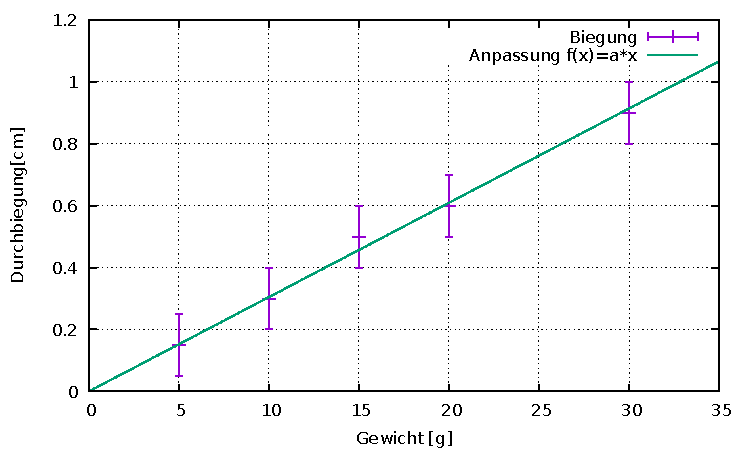
\includegraphics[width=1\textwidth]{res/DurchbiegungAlu.pdf}
	\caption{Zu sehen ist hier die Durchbiegung des Runden Aluminiumstabes in Abhängigkeit vom Gewicht.}
	\label{fig:durchbiegungalu}
\end{figure}

\begin{figure}[h]
	\centering
	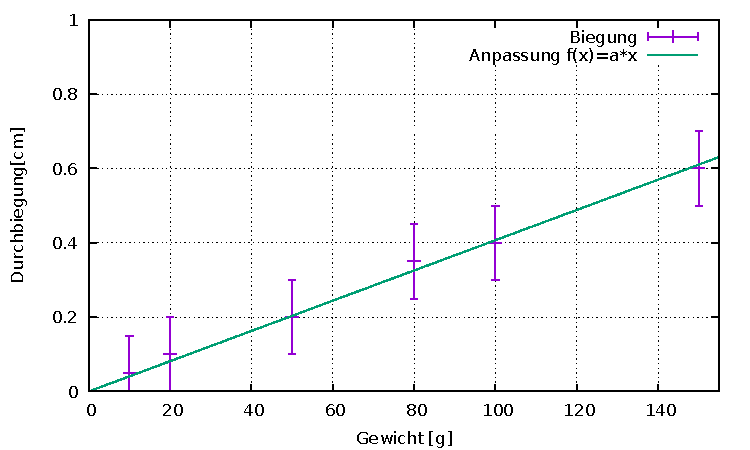
\includegraphics[width=1\textwidth]{res/DurchbiegungMessingHochkant.pdf}
	\caption{Zu sehen ist hier die Durchbiegung des Hochkant gestellten rechteckigen Messingstabes in Abhängigkeit vom Gewicht.}
	\label{fig:durchbiegungMessHoch}
\end{figure}

\begin{figure}[h]
	\centering
	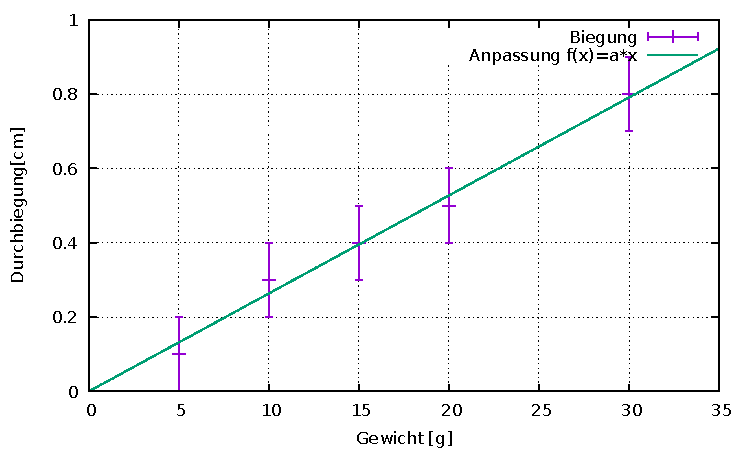
\includegraphics[width=1\textwidth]{res/DurchbiegungMessingQuer.pdf}
	\caption{Zu sehen ist hier die Durchbiegung des Quer gestellten rechteckigen Messingstabes in Abhängigkeit vom Gewicht.}
	\label{fig:durchbiegungMessQuer}
\end{figure}

\begin{figure}[h]
	\centering
	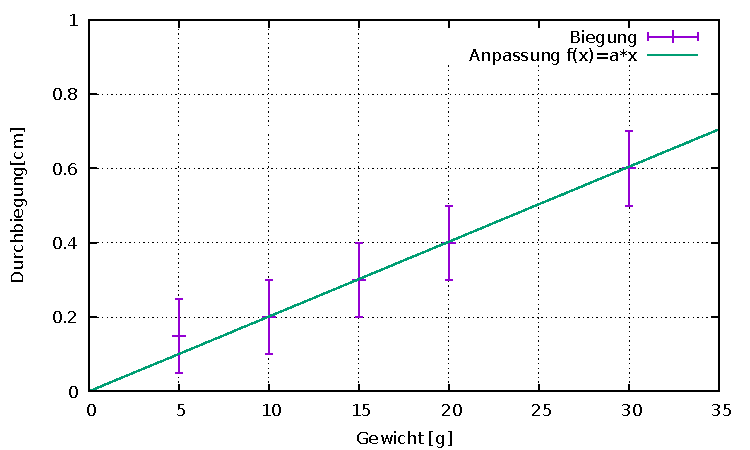
\includegraphics[width=1\textwidth]{res/DurchbiegungMessingRund.pdf}
	\caption{Zu sehen ist hier die Durchbiegung des Runden Messingstabes in Abhängigkeit vom Gewicht.}
	\label{fig:durchbiegungMessRund}
\end{figure}

\begin{figure}[h]
	\centering
	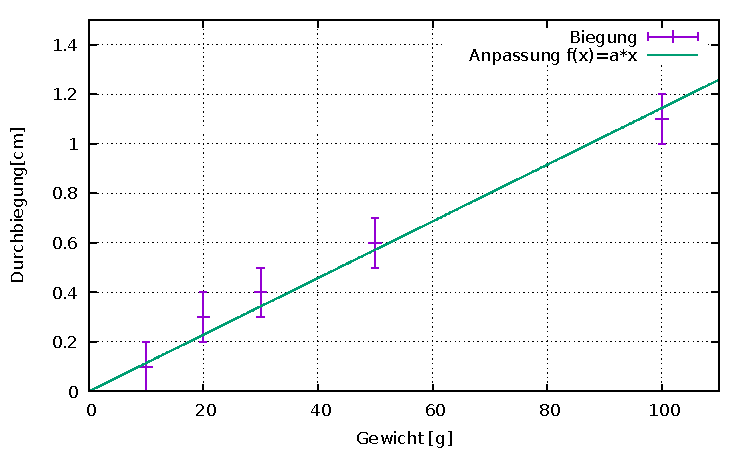
\includegraphics[width=1\textwidth]{res/DurchbiegungStahl.pdf}
	\caption{Zu sehen ist hier die Durchbiegung des Runden Stahlstabes in Abhängigkeit vom Gewicht.}
	\label{fig:durchbiegungStahl}
\end{figure}
\begin{table}[h]
	\caption{Literaturwerte für das Elastizitätsmodul}
	\begin{tabular}{|c|c|}
		\hline
		& Elastizitätsmodul E $\left[\frac{GN}{m^2}\right]$\\
		\hline
		Aluminium & 70 \\
		\hline
		Eisen & 190 \\
		\hline
		Kupfer & 110 \\
		\hline
		Messing & 90 \\
		\hline
	\end{tabular}
\label{tab:ElaLit}
\end{table}